%Siehe "`Raytracing from Ground Up"' S. 217


\chapter{Schattierung} \label{ch:schattierung}


Bis jetzt ist der "`Raytracer"' in der Lage Strahlen in eine Szene bestehend aus Objekten auszusenden und Schnittpunkte zu berechnen. An diesen Schnittpunkten muss nun ein Farbwert berechnet werden, der anschließend dem PEE zugewiesen wird, welches vom Strahl durchdrungen wurde. Den Vorgang zur Berechnung des Farbwerts bezeichnet man in der Computergrafik als Schattierung. 


\section{Die Rendergleichung}

Beim "`Raytracing"' erfolgt die Schattierung eines Objekts durch Lösung der Rendergleichung. Der Farbwert ergibt sich aus der Summe aller, über der Hemisphäre eines Schnittpunktes, einfallender Strahldichten. Dabei entscheidet der Einfallwinkel und der Schnittpunkt, welche Frequenzanteile, einer einfallenden Strahldichte, mit welcher Intensität entlang eines Primärstrahls auf das PEE reflektiert wird. Zur Modellierung dieses Sachverhalts verwendet man bidirektionale Reflektanzverteilungsfunktionen (engl. bidirectional reflectance distribution function, BRDF\abk{BRDF}{Bidirectional reflectance distribution function}). Die BRDF ist damit maßgeblich für die Oberflächeneigenschaft und somit für die Schattierung eines Objekts verantwortlich.

\begin{equation}
    L_o(\boldsymbol{p}, \boldsymbol{\omega_o}) = L_e(\boldsymbol{p}, \boldsymbol{\omega_o}) + \int_{2\pi^+} f_r(\boldsymbol{p}, \boldsymbol{\omega_i}, \boldsymbol{\omega_o}) \cdot L_i(\boldsymbol{p}, \boldsymbol{\omega_i}) \cos(\theta_i) \mathrm{d} \boldsymbol{\omega_i}
    \label{eq:rendergleichung}
\end{equation}

Gleichung~\ref{eq:rendergleichung} zeigt die Rendergleichung. Der Term \( L_o(\boldsymbol{p}, \boldsymbol{\omega_o}) \) steht dabei für die, aus der Oberfläche austretende Strahldichte. Dieser Term ist wie bereits erwähnt abhängig vom Schnittpunkt \( \boldsymbol{p} \) und der Strahlrichtung \( \boldsymbol{\omega_o} \), die der inversen Richtung des Primärstrahls entspricht. Der Term \( L_e(\boldsymbol{p}, \boldsymbol{\omega_o}) \) wird für Oberflächen benötigt, die selbst Licht emittieren. Der restliche Summenteil der ausgehenden Strahldichte ergibt sich, indem man über alle möglichen Strahlrichtungen \( \boldsymbol{\omega_i} \) in der Hemisphäre integriert, die sich über dem Schnittpunkt \( \boldsymbol{p} \) befindet. Die einfallenden Strahldichten \( L_i(\boldsymbol{p}, \boldsymbol{\omega_i}) \), werden wie erwähnt durch die BRDF \( f_r(\boldsymbol{p}, \boldsymbol{\omega_i}, \boldsymbol{\omega_o}) \) skaliert. Zuletzt fehlt noch der Ausdruck \( \cos(\theta_i) \), der dafür sorgt, dass flacher einfallende Strahldichten einen geringeren Beitrag zur ausgehenden Strahldichte leisten, als steiler einfallende. Der Winkel \( \theta_i \) lässt sich aus der Normale \( \boldsymbol{n} \) am Schnittpunkt \( \boldsymbol{p} \) und der Strahlrichtung \( \boldsymbol{\omega_i} \), eines einfallenden Strahls, berechnen.

Die Rendergleichung kann in der Regel nicht analytisch gelöst werden und muss daher approximiert werden. Eine Variante besteht darin, Strahlen gemäß einer Verteilung (z.B. gleichverteilt) über der Hemisphäre, in die Szene zu schicken, um konkrete Werte für \( L_i(\boldsymbol{p}, \boldsymbol{\omega_i}) \) zu berechnen. Trifft einer dieser Strahlen auf ein Objekt wird das Verfahren rekursiv fortgesetzt, bis eine Lichtquelle getroffen wird. Dieses Vorgehen nennt man "`Path Tracing"' und kann für kleine Lichtquellen sehr lange dauern, da Strahlen diese nur selten treffen. Für unendlich viele ausgesandte Strahlen, stellt "`Path Tracing"' jedoch eine korrekte Lösung der Rendergleichung da.

Beim "`Whitted Raytracing"' wird hingegen für jeden Primärstrahl, der ein Objekt trifft, der Term \( L_i(\boldsymbol{p}, \boldsymbol{\omega_i)} \) berechnet, indem Strahlen nur zu allen in der Szene befindlichen Lichtquellen ausgesandt werden. Diese Methode ist deutlich schneller, stellt jedoch nur eine sehr ungenaue Approximation der Rendergleichung da. Die folgenden Abschnitte zeigen, wie Objekte nach der "`Whitted"' Methode schattiert werden können.


\section{Matte Oberfläche}

\begin{wrapfigure}{r}{0.5\textwidth}    
    \vspace{-15pt}
    \centering
    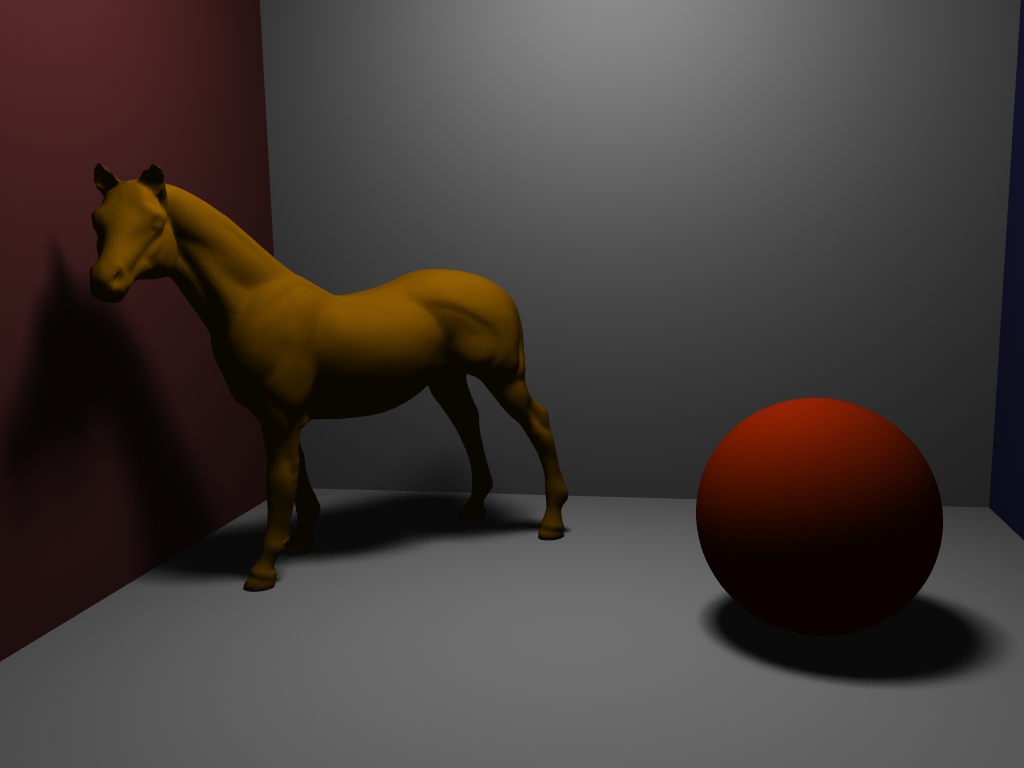
\includegraphics[width=0.49\textwidth]{img/schattierung/matte_0,05_0,85.png}
    \vspace{-10pt}
    \caption{Pferdemodell und Kugel in einer Box  }
    \label{fig:matte_0,05_0,85.png}
\end{wrapfigure}

Matte oder "`lambertsche"' Oberflächen besitzen eine sehr einfache Schattierung. Sie bestehen im Wesentlichen aus zwei Komponenten und zwar aus einem ambienten und einem diffusen Term:

\( f_{matt}(\boldsymbol{p}, \boldsymbol{\omega_i}, \boldsymbol{\omega_o}) = k_a \cdot c_a + k_d \cdot c_d \)

 Der ambiente Term ist unabhängig vom Austrittswinkel \( \omega_o \) und dem Einfallswinkel \( \omega_i \). Da beim "`Whitted Raytracing"' die Lichtausbreitung zwischen nicht-Licht emittierenden Objekten fehlt, soll er den Eindruck von vorhandenem Umgebungslicht vermitteln. Bei \( k_a \) handelt es sich um den ambienten Reflexionskoeffizienten \( k_a \). Er bestimmt den Anteil der ambienten Komponente in der ausgehenden Strahldichte. Die Materialkonstante \( c_a \), sorgt für die Färbung des Objekts, indem sie bestimmte Spektren absorbiert und andere reflektiert. Wird \( c_a \) als RGB-Wert dargestellt, so entspricht dies einer Multiplikation mit dem RGB-Wert der einfallenden Strahldichte. Für die diffuse Komponente sind die Bedeutungen von \( k_d \text{ und } c_d \) analog. In der gerasterten Computergrafik wird für die matte Oberflächen noch ein Term benötigt, der die Intensität eines Farbwertes skaliert, je nachdem wie flach oder steil ein Strahl von der Lichtquelle auf die Oberfläche trifft. Beim "`Raytracing"' ist dieser Sachverhalt bereits durch \( \cos{\theta_i} \), in der Rendergleichung, modelliert
 

\section{Spekulare Oberfläche - Phong}

Für spekulare Oberflächen muss die matte Schattierung um eine weitere Komponente ergänzt werden. Diese Komponente ist verantwortlich für die Darstellung von Glanzpunkten und wird Phong-Komponente genannt:

\begin{equation*}
f_{phong}(\boldsymbol{p}, \boldsymbol{\omega_i}, \boldsymbol{\omega_o}) = f_{matt}(\boldsymbol{p}, \boldsymbol{\omega_i}, \boldsymbol{\omega_o}) + \left( \frac{\boldsymbol{\omega_o} \cdot \boldsymbol{r} }{|\boldsymbol{\omega_o}| \cdot |\boldsymbol{r}|} \right)^n \cdot k_p \cdot c_p
\end{equation*}

Bei den Konstanten \( k_p \) und \( c_p \) handelt es sich um den  Reflexionskoeffizienten und die Materialkonstante. Diese werden mit einem Term multipliziert, der den Winkel zwischen ausgehender Strahlrichtung \( \boldsymbol{\omega_o} \) und einem Vektor \( \boldsymbol{r} \) berechnet. Bei \( \boldsymbol{r} \) handelt es sich um die perfekte Reflexionsrichtung, eines einfallenden Lichtstrahls. Er wird erzeugt durch 

\( \boldsymbol{r} = -\boldsymbol{\omega_i} \cdot 2 \cdot (\boldsymbol{n} \cdot \boldsymbol{\omega_i}) \cdot \boldsymbol{n}\), wobei Normale \( \boldsymbol{n} \) und \( \boldsymbol{\omega_i} \) normalisiert sein müssen. Je weiter der Winkel zwischen Beobachter und perfekt reflektiertem Lichtstrahl ist, desto geringer ist der Anteil der Phong-Komponenten an der ausgehenden Strahldichte. Der Exponent \( n \) wird dazu verwendet die Ausdehnung der Glanzpunkte festzulegen, wie Abb.~\ref{fig:phong_30} und Abb.~\ref{fig:phong_100} zeigen. Je größer \( n \) ist, desto konzentrierter erscheinen die Glanzpunkte.

\begin{minipage}[t]{0.48\textwidth}
    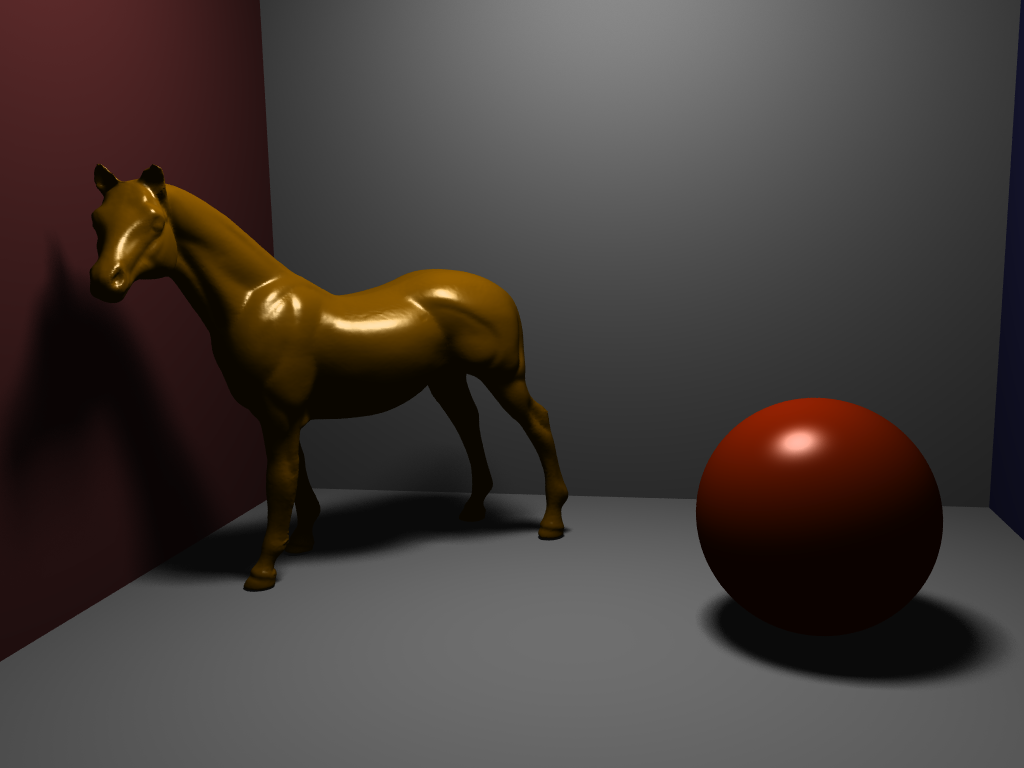
\includegraphics[width=\textwidth]{./img/schattierung/phong_30.png}
    \captionof{figure}{Pferd und Kugel mit spekularer Oberfläche. Die Größen der Glanzpunkte ergeben sich durch den Exponenten $n=30$.}
    \label{fig:phong_30}
\end{minipage}
\begin{minipage}[t]{0.48\textwidth}
    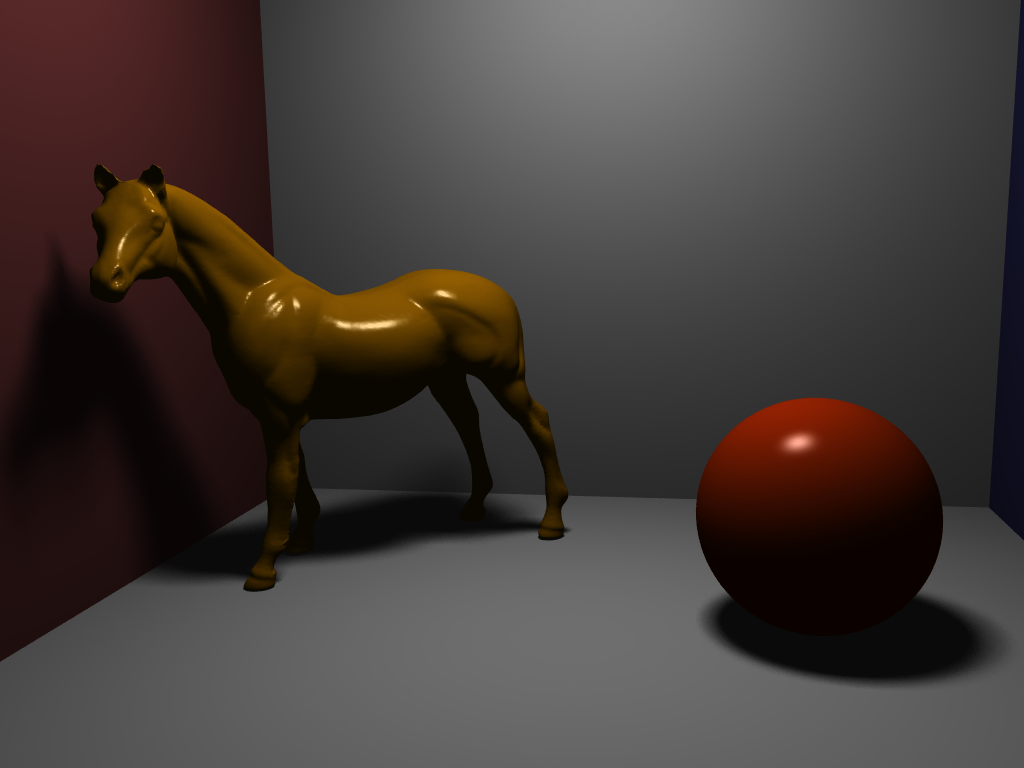
\includegraphics[width=\textwidth]{./img/schattierung/phong_100.png}
    \captionof{figure}{Pferd und Kugel mit spekularer Oberfläche. Die Größen der Glanzpunkte ergeben sich durch den Exponenten $n=100$.}
    \label{fig:phong_100}
\end{minipage}

\section{Spiegelnde Oberfläche}

Die Spiegeloberflächen aus Abb.~\ref{fig:rmirror_100exp} und Abb.~\ref{fig:mirror} stellen eine Erweiterung der Phong-Schattierung da. Jedoch sollten die ambiente, diffuse und Phong-Komponente sehr dezent eingesetzt werden. Perfekte Reflexion kann umgesetzt werden, indem ein Strahl in Richtung perfekter Reflexionsrichtung \( \boldsymbol{r} \) ausgesandt wird. Trifft er ein anderes Objekt, wird dort am Schnittpunkt die Schattierungsberechnung durchgeführt und die Strahldichte berechnet. Die dort berechnete Strahldichte kann dann anhand eines weiteren additiven Terms bestehend aus Reflexionskoeffizient und Materialkonstante verändert und zur ausgehenden Strahldichte der perfekt spiegelnden Oberfläche hinzugefügt werden.

Abb.~\ref{fig:phong_30} zeigt eine matt spiegelnde Oberfläche. Dies erreicht man, indem man Strahlen konisch verteilt, entlang von \( \boldsymbol{r} \) in die Szene schickt.



\begin{minipage}[t]{0.48\textwidth}
    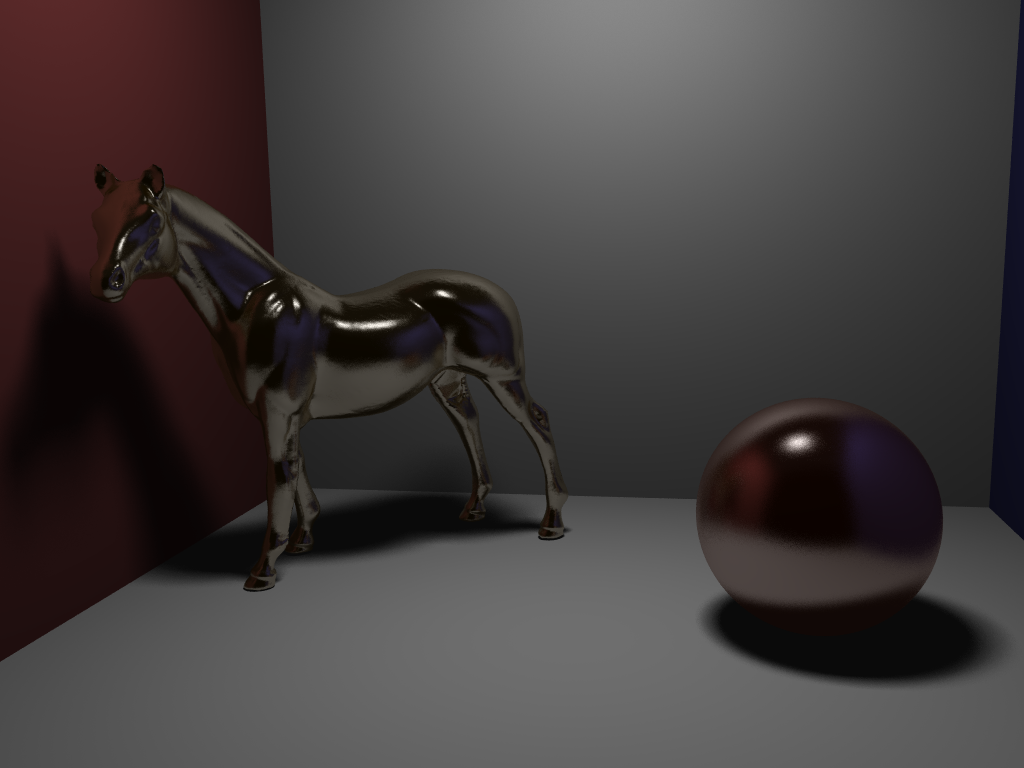
\includegraphics[width=\textwidth]{./img/schattierung/rmirror_100exp.png}
    \captionof{figure}{Das Aussehen der matt spiegelnden Oberflächen wird erzeugt, indem Strahlen konisch um die perfekte Reflexionsrichtung $\boldsymbol{r}$ in die Szene geschickt werden.}
    \label{fig:rmirror_100exp}
\end{minipage}
\begin{minipage}[t]{0.48\textwidth}
    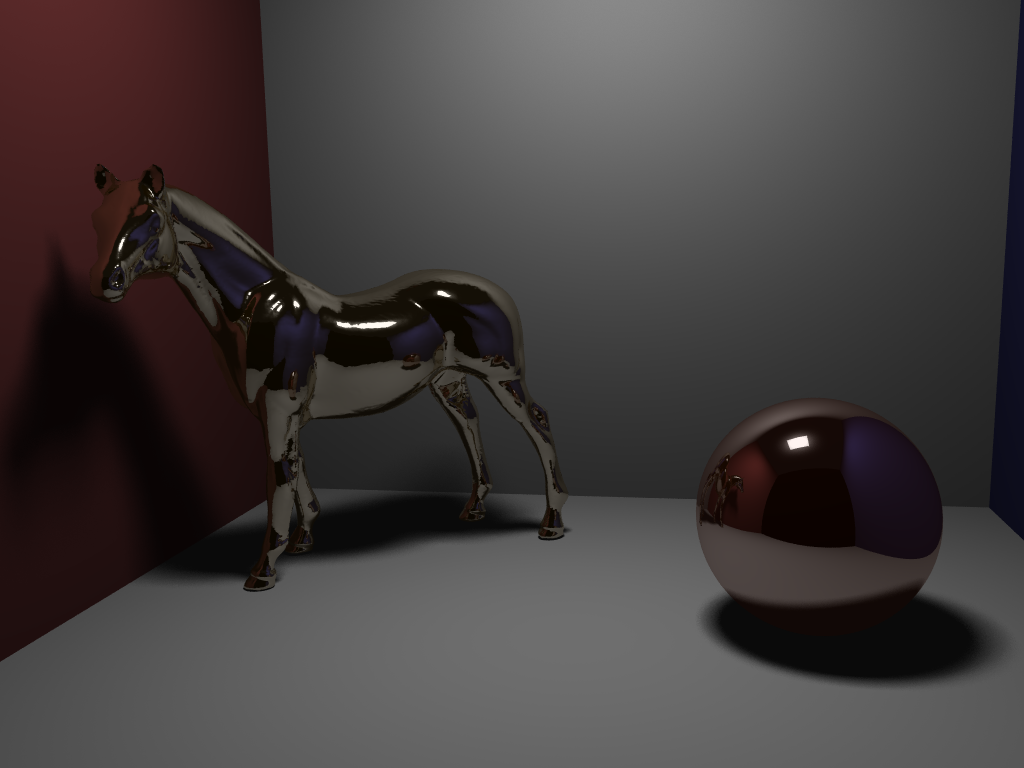
\includegraphics[width=\textwidth]{./img/schattierung/mirror.png}
    \captionof{figure}{Das Aussehen der perfekt spiegelnden Oberflächen wird erzeugt, indem Strahlen entlang der perfekten Reflexionsrichtung $\boldsymbol{r}$ in die Szene geschickt werden.}
    \label{fig:mirror}
\end{minipage}


\section{Dielektrikum}

Bei Dielektrika handelt es sich um Materialien, die Anteile eines eintreffenden Lichtstrahls brechen und reflektieren. Jedes Dielektrikum besitzt einen Brechungsindex. Mit Hilfe des Snelliusschen Brechungsgesetz und des Brechungsindex kann bestimmt werden, in welche Richtung ein Strahl gebrochen wird, wenn er vom umgebenden Medium in das Dielektrikum übergeht. Wenn ein Strahl zu flach auf die Oberfläche auftrifft, kann es passieren, dass er komplett reflektiert wird und muss dann wie bei perfekt spiegelnden Oberflächen behandelt werden. Man spricht in diesem Fall von Totalreflexion. Findet keine Totalreflexion statt, wird ein Teil des Strahls gebrochen und ein Teil reflektiert. Durch die Fresnelschen Formeln kann dann bestimmt werden, aus welchen Anteilen der Strahldichte des gebrochenen Strahls und des reflektierten Strahls, sich die ausgehende Strahldichte zusammensetzt.  

\begin{minipage}[t]{0.48\textwidth}
    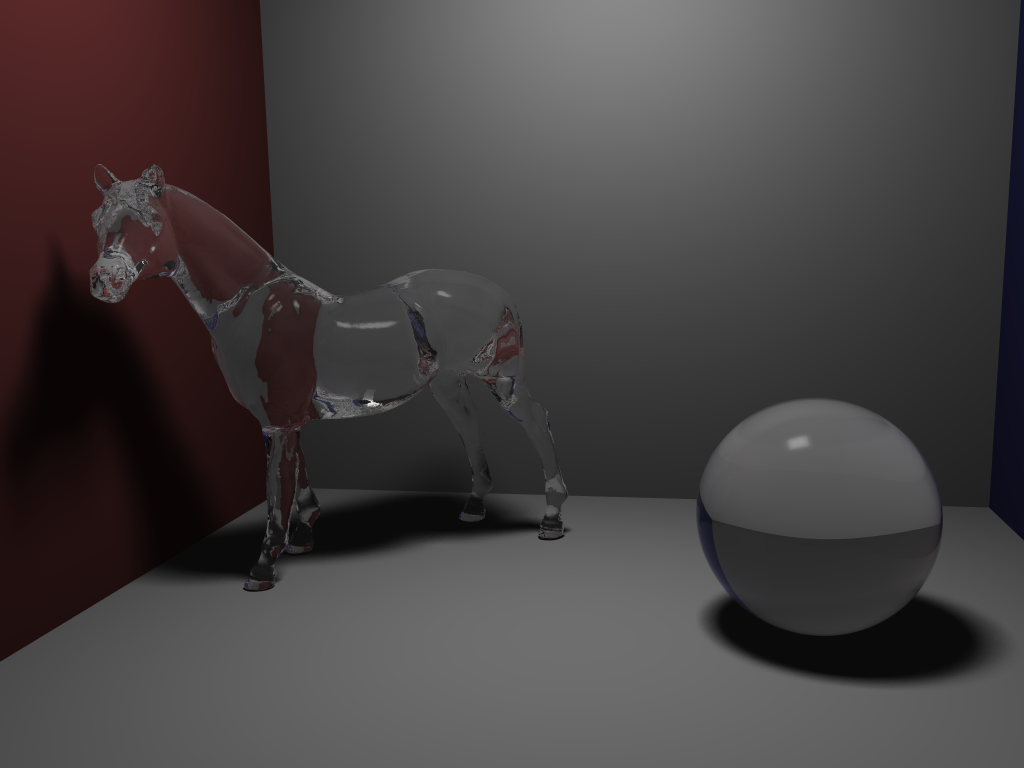
\includegraphics[width=\textwidth]{./img/schattierung/dielectric_1_1,3.png}
    \captionof{figure}{Dielektrika mit einem Brechungsindex von 1,3. Dies entspricht näherungsweise dem Übergang von Luft zu Eis}
    \label{fig:dielectric_1_1,3.png}
\end{minipage}
\begin{minipage}[t]{0.48\textwidth}
    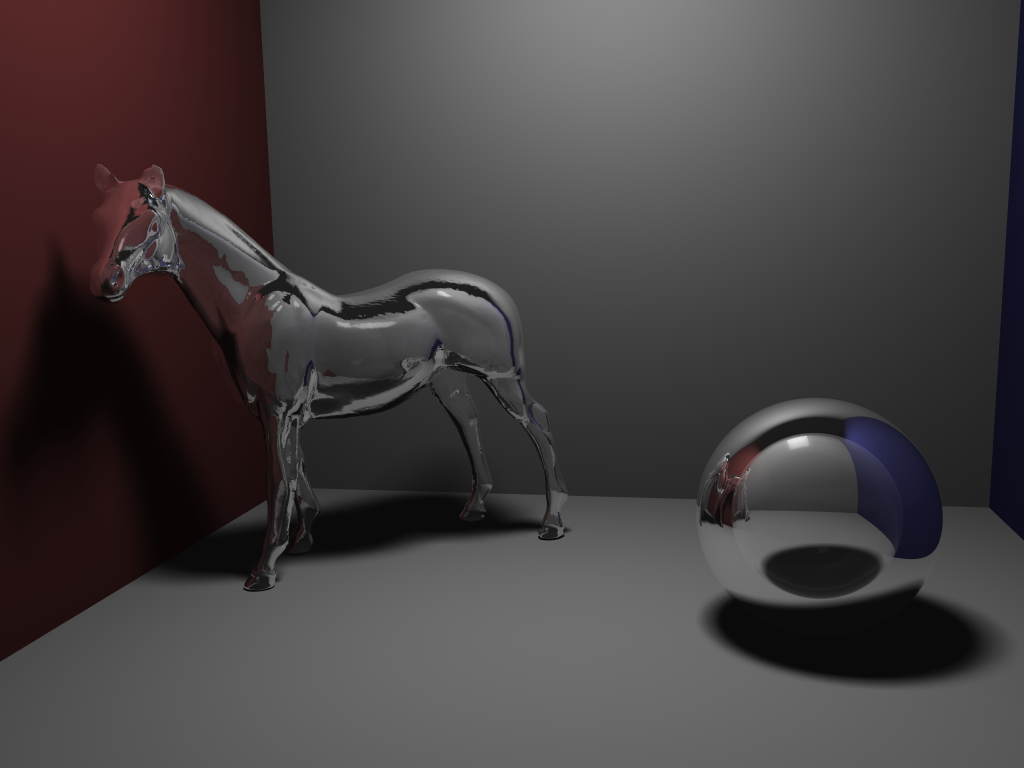
\includegraphics[width=\textwidth]{./img/schattierung/dielectric_1_0,7.png}
    \captionof{figure}{Dielektrika mit einem Brechungsindex von 0,75. Dies entspricht näherungsweise dem Übergang von Wasser zu Luft}
    \label{fig:dielectric_1_0,7.png}
\end{minipage}

